\documentclass{beamer}
\usetheme{Madrid}

\usepackage[utf8]{inputenc}
\usepackage{subfig}
\usepackage{tikz}   
\captionsetup[subfloat]{labelformat=empty}



\title[FGNs vs Adversarial Attacks] %optional
{Finite Gaussian Neurons}
\subtitle{A Defense Against Adversarial Attacks?}

\author[Felix Grezes] % (optional, for multiple authors)
{Felix Grezes}

\institute[CUNY GC] % (optional)
{
  \inst{}%
  Graduate Center\\
  City University of New York
}

\date[Thesis Proposal - Fall 2020] % (optional)
{Thesis Proposal Fall 2020}

\logo{
\includegraphics[height=1.5cm]{images/gc_logo_286_3_300px_511px.png}}

\begin{document}

\frame{\titlepage}

\begin{frame}
    \frametitle{Table of Contents}
    \tableofcontents
\end{frame}


\section{Abstract}
\begin{frame}{Abstract}
I introduce the Finite Gaussian Neuron, a novel neural network architecture.\\

My works aims to:
\begin{itemize}
    \item make it easy to convert existing models to the FGN architecture
    \item while preserving the existing model's behavior on real data
    \item and offering resistance against some adversarial attacks.
\end{itemize}

\end{frame}


\section{Introduction}
\begin{frame}{Introduction}
    
\end{frame}


\section{Related Work}
\begin{frame}{Related Work}
    
\end{frame}


\section{Motivation}
\begin{frame}{Motivation}

\end{frame}


\section{The Finite Gaussian Neuron}

\begin{frame}{The Classical Neuron}
    % Classic neuron math
    \begin{block}{Neuron Output}
        $$y = \varphi(\ell)$$
    \end{block}
    \begin{block}{Linear Component}
        $$\ell=\sum_i x_i w_i$$
    \end{block}
    % classic neuron illustrated
    \begin{center}
        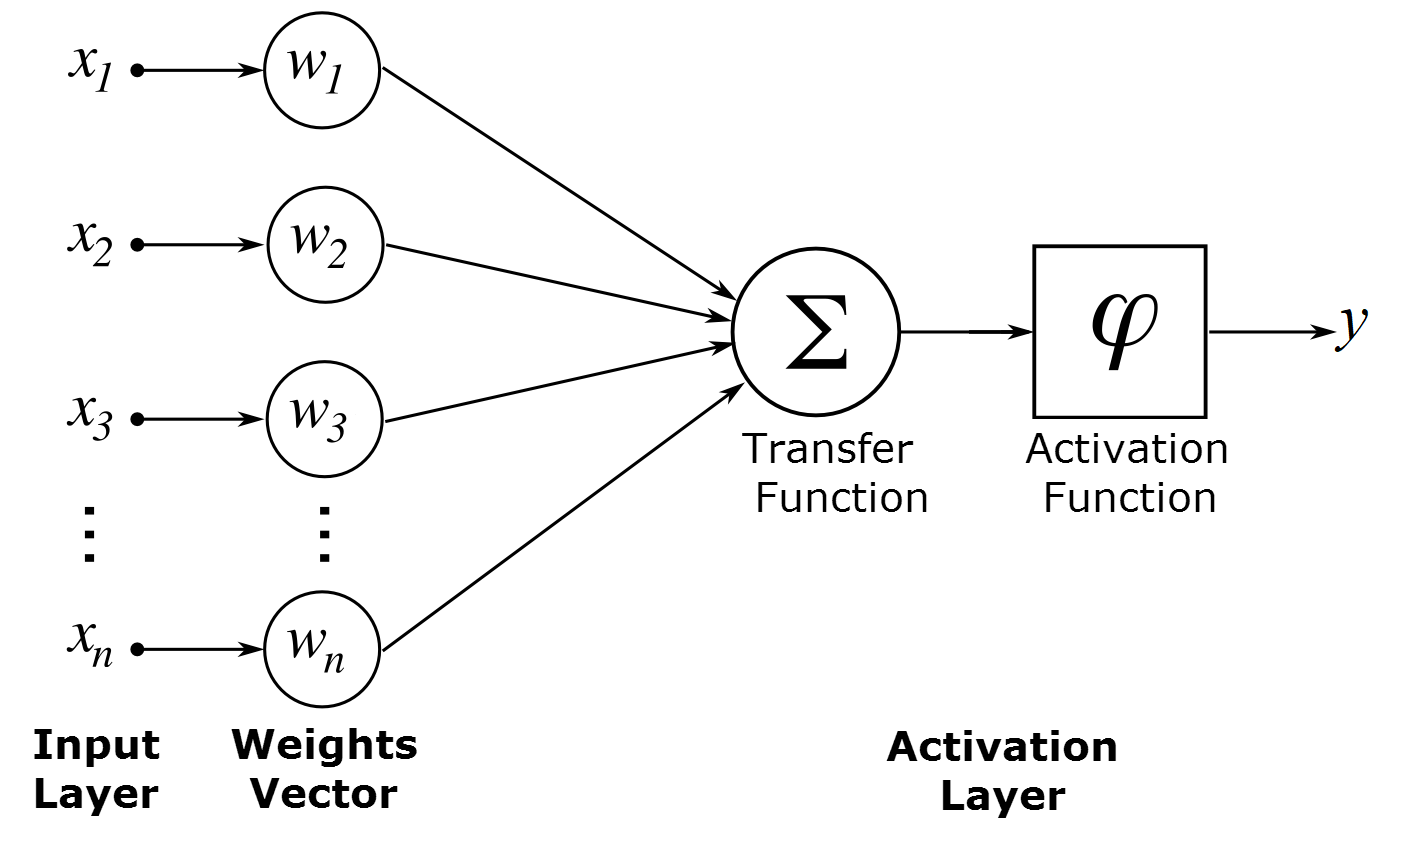
\includegraphics[width=0.6\textwidth]{images/artificial_neuron_model.png}
    \end{center}
\end{frame}

\begin{frame}{The Finite Gaussian Neuron}
    %%math
    \begin{block}{Neuron Output}
        $$ y =  \varphi(\ell)*g = \varphi(\sum_i x_i w_i) * g$$
    \end{block}
    \begin{block}{Gaussian Component}
    % $$ g = exp \left( \frac{-1}{\sigma^2}*\sum_{i}(x_i-c_i)^2 \right)$$
    % $$ g = exp(\frac{-\sum_i (x_i-c_i)^2}{\sigma^2} )$$
    $$ g = e^{\frac{-1}{\sigma^2}\sum_{i}(x_i-c_i)^2}$$
    \end{block}
    %% gaussian component illustrated
    \begin{center}
        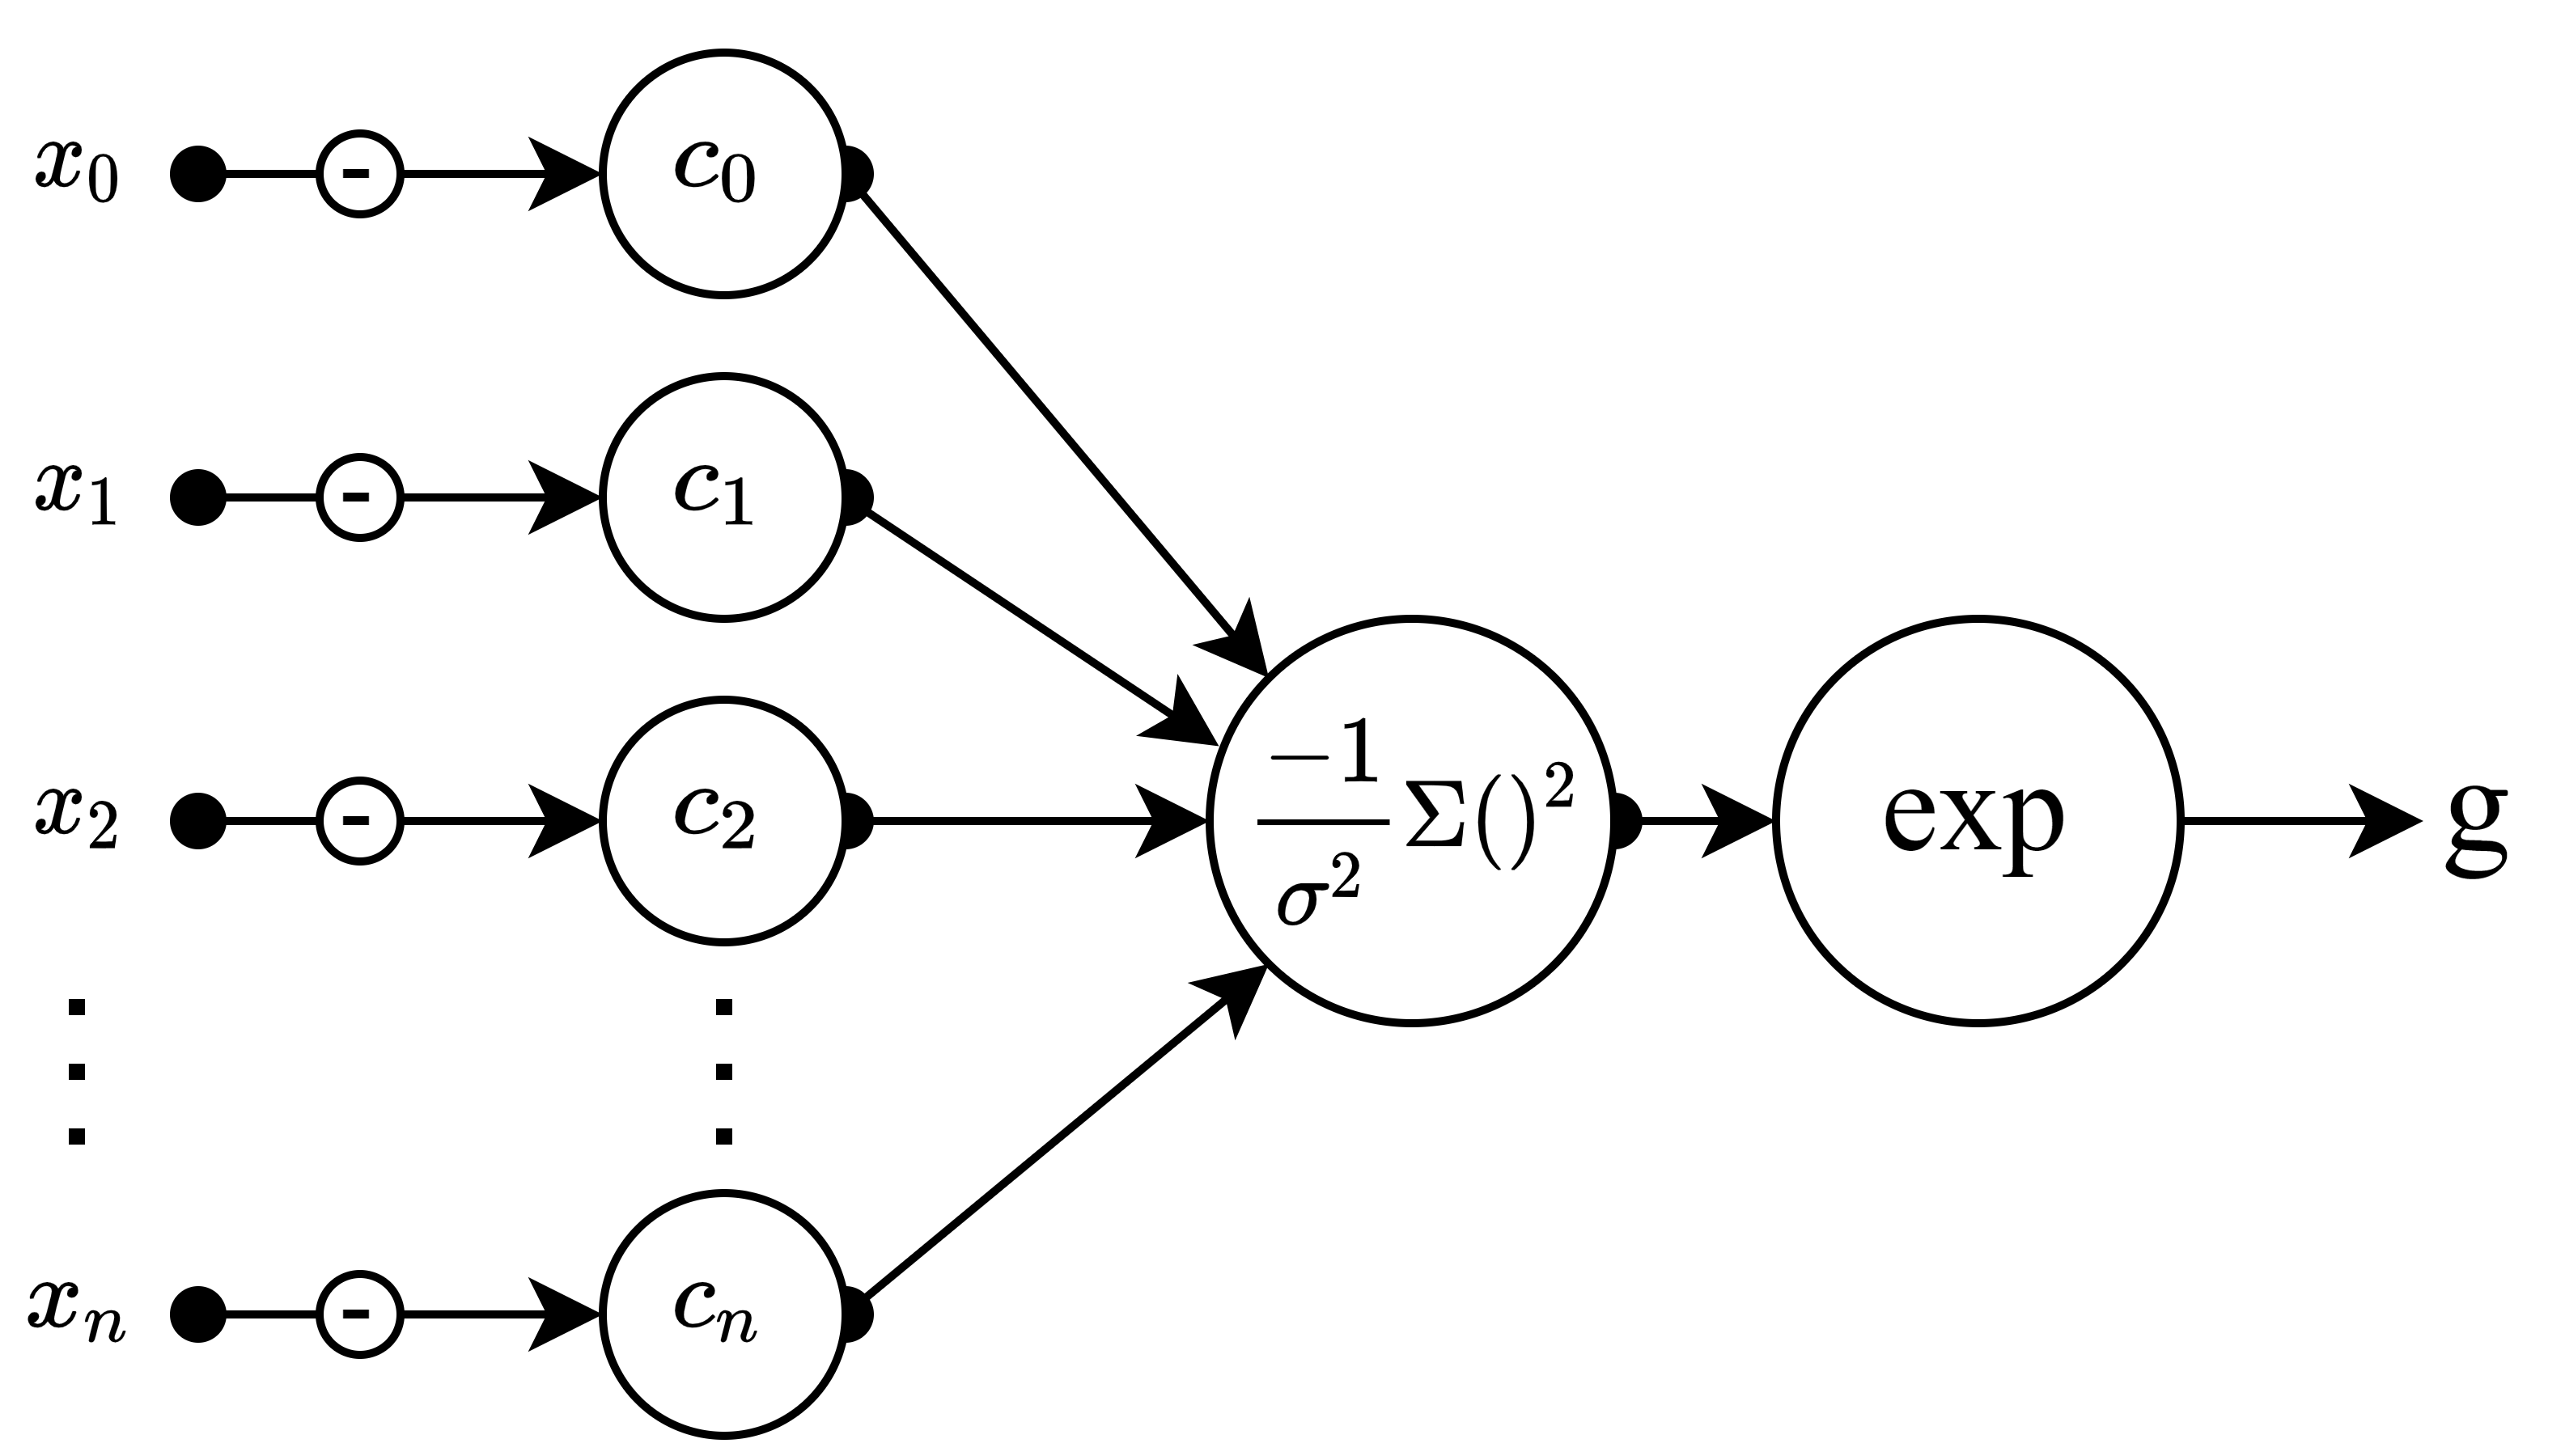
\includegraphics[width=0.5\textwidth]{images/fgn-gaussian-component.png}
    \end{center}
\end{frame}

\begin{frame}{2D Neuron Activity Visualization}
    % 2 images for classic: linear and after non-linearity like tanh
    % 2 images for fgn: gaussian component and combination 
    \vspace{-0.5cm}
    \begin{figure}
      \centering
      \subfloat[Linear: $\ell = W^tX$]{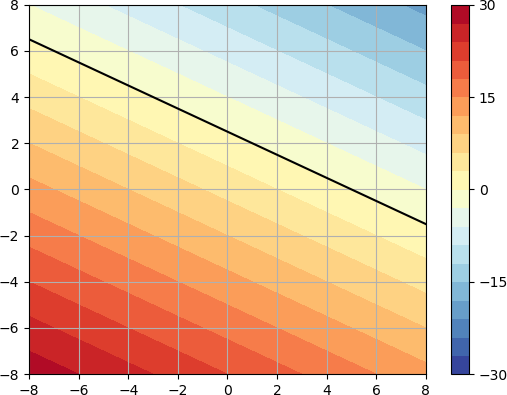
\includegraphics[height=3.2cm,width=4cm]{images/2D Activity/2d-linear-activity-cropped.png}} \hspace{0.5cm}
      \subfloat[Classic: $y = \tanh(\ell)$]{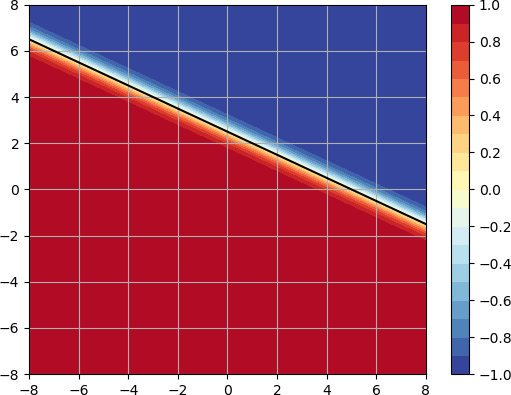
\includegraphics[height=3.2cm,width=4cm]{images/2D Activity/2d-classic-activity-cropped.png}}\\
      \vspace{-0.2cm}
      \subfloat[$g = e^{\frac{-1}{\sigma^2}*\sum_{i}(x_i-c_i)^2}$]{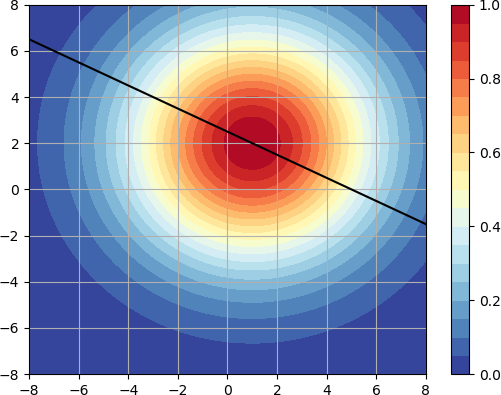
\includegraphics[height=3.2cm,width=4cm]{images/2D Activity/2d-gaussian-activity-cropped.png}} \hspace{0.5cm}
      \subfloat[FGN: $y = \tanh(\ell)*g$]{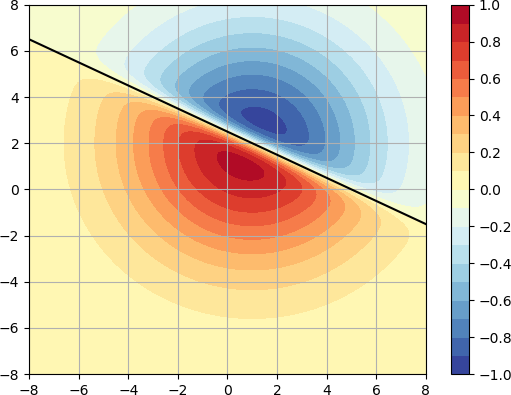
\includegraphics[height=3.2cm,width=4cm]{images/2D Activity/2d-fgn-activity-cropped.png}}
    \end{figure}
\end{frame}

\begin{frame}{Matching Classical Neuron Behavior}
    \begin{block}{Property}
    As $\sigma$ increases, the Finite Gaussian Neuron's behavior gets closer that of the classical neuron with the same $W$ weights.
    \end{block}
    \vspace{0.2cm}
    \begin{tikzpicture}
        \node (img1) {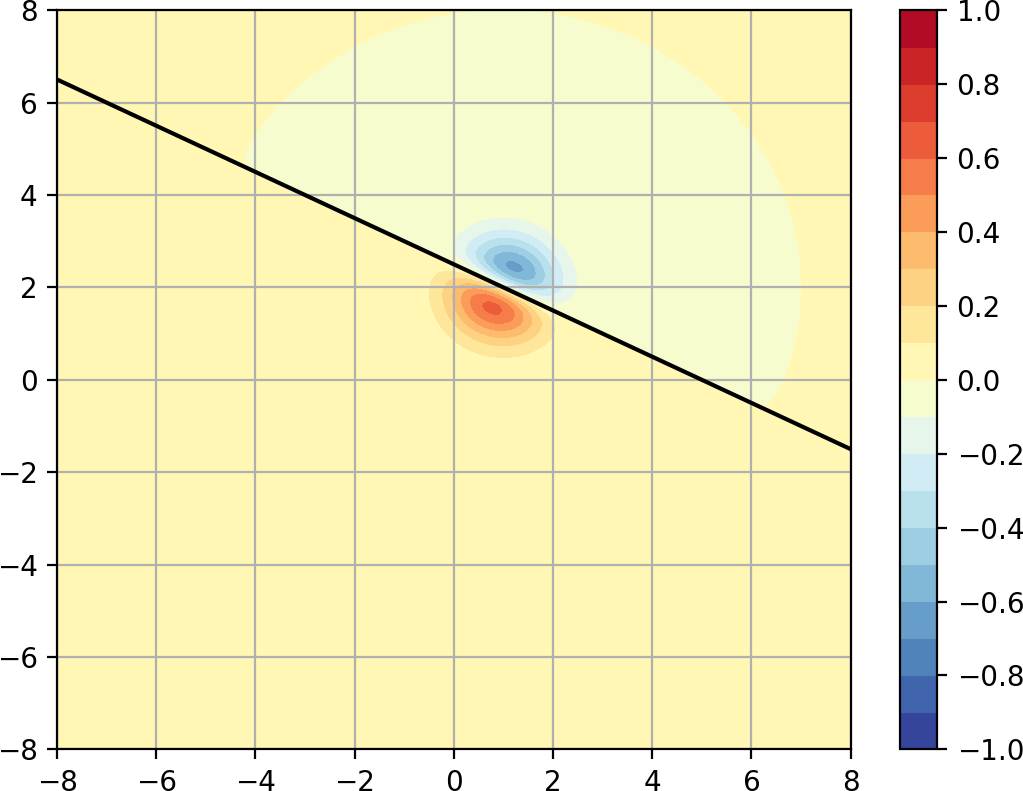
\includegraphics[height=3cm]{images/Matching-behavior/sigma-1-cropped.png}};\pause
        \node (img2)at(img1.south east) [xshift=-0.75cm]{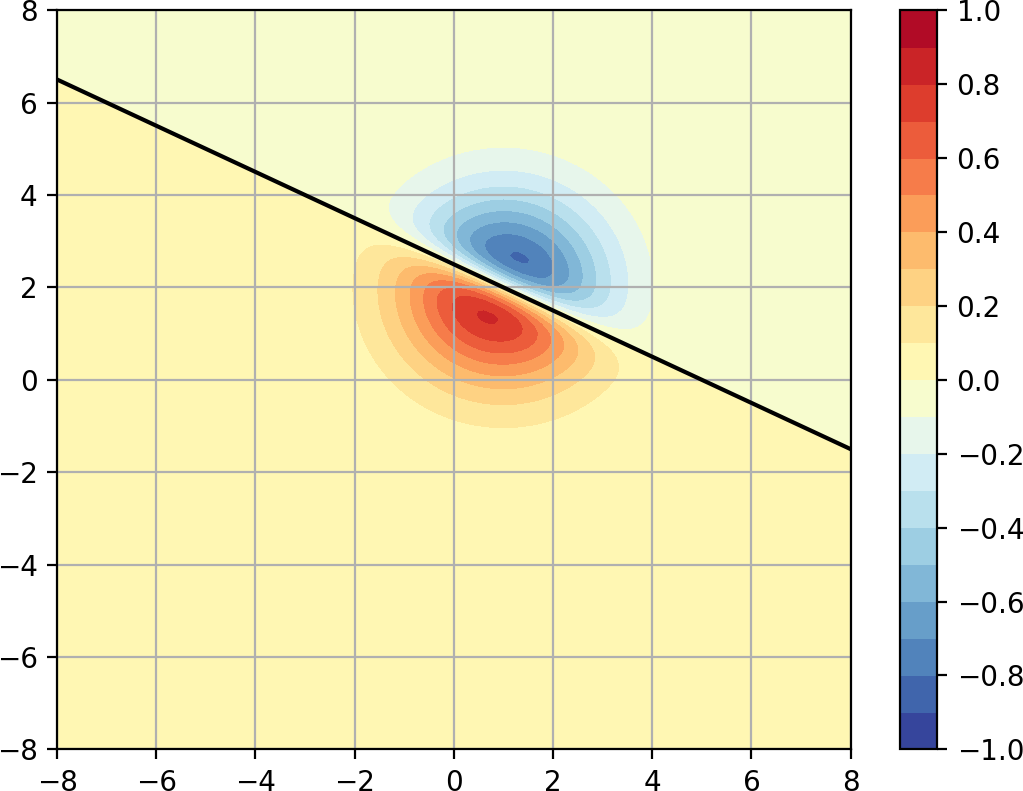
\includegraphics[height=3cm]{images/Matching-behavior/sigma-2-cropped.png}};\pause
        \node (img3)at(img2.north east) [xshift=-0.75cm]{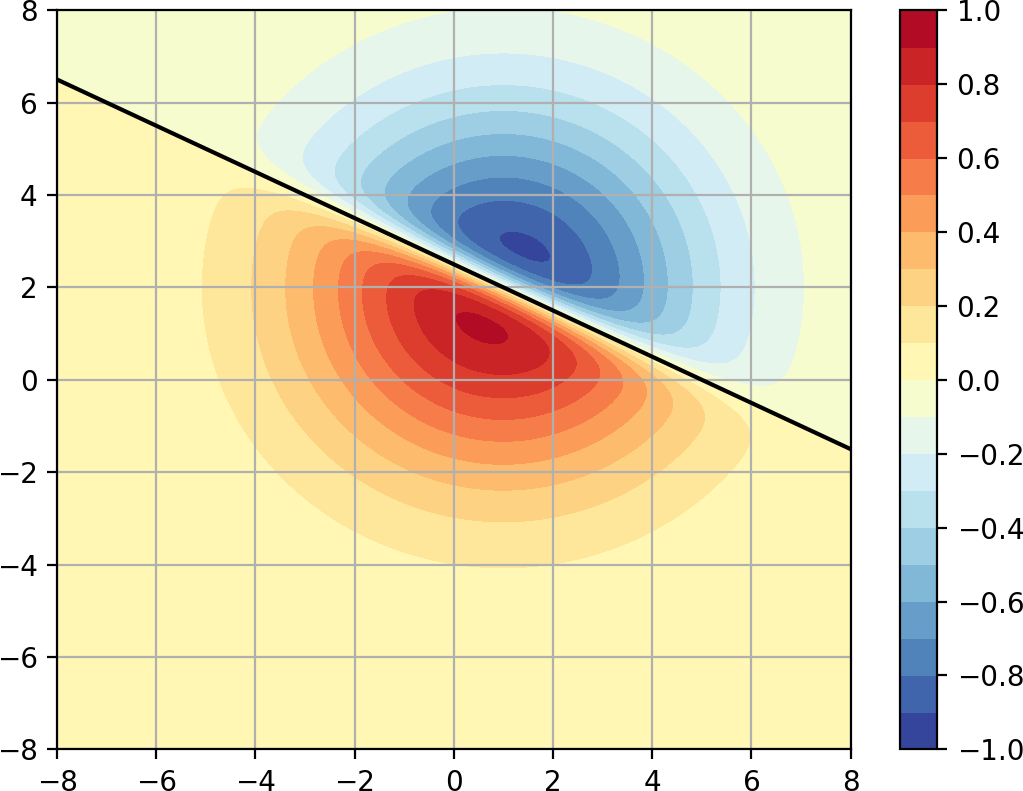
\includegraphics[height=3cm]{images/Matching-behavior/sigma-3-cropped.png}};\pause
        \node (img4)at(img3.south east) [xshift=-0.75cm]{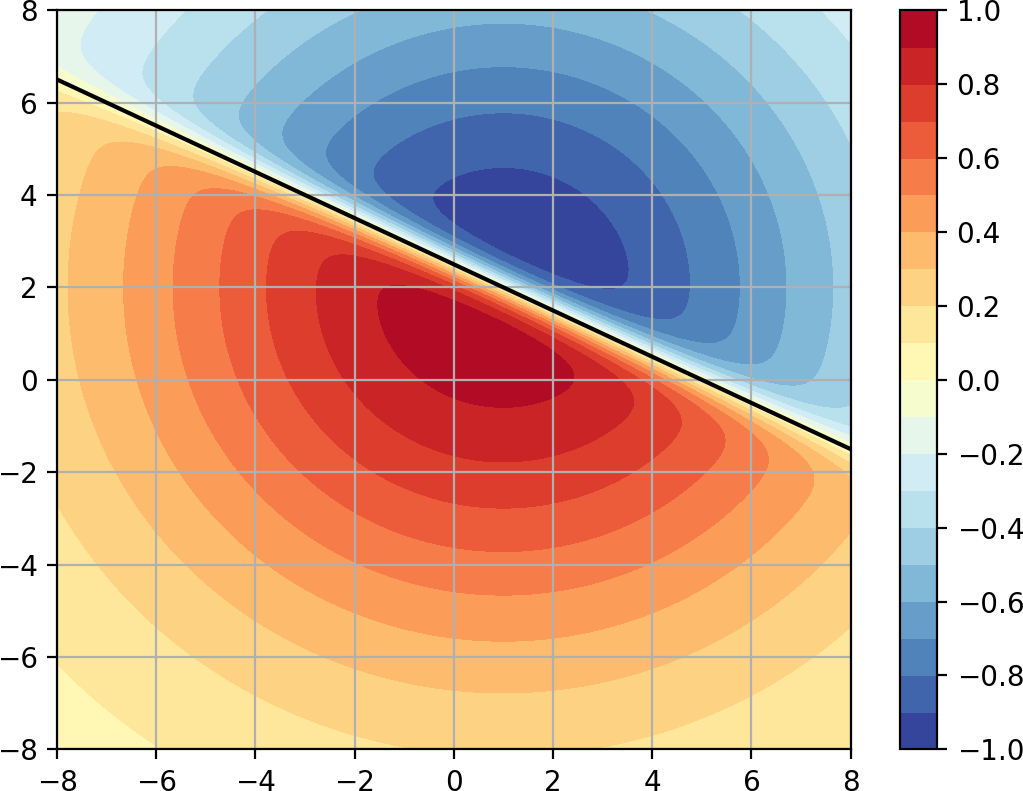
\includegraphics[height=3cm]{images/Matching-behavior/sigma-4-cropped.png}};\pause
        \node (img5)at(img4.north east) [xshift=-0.75cm]{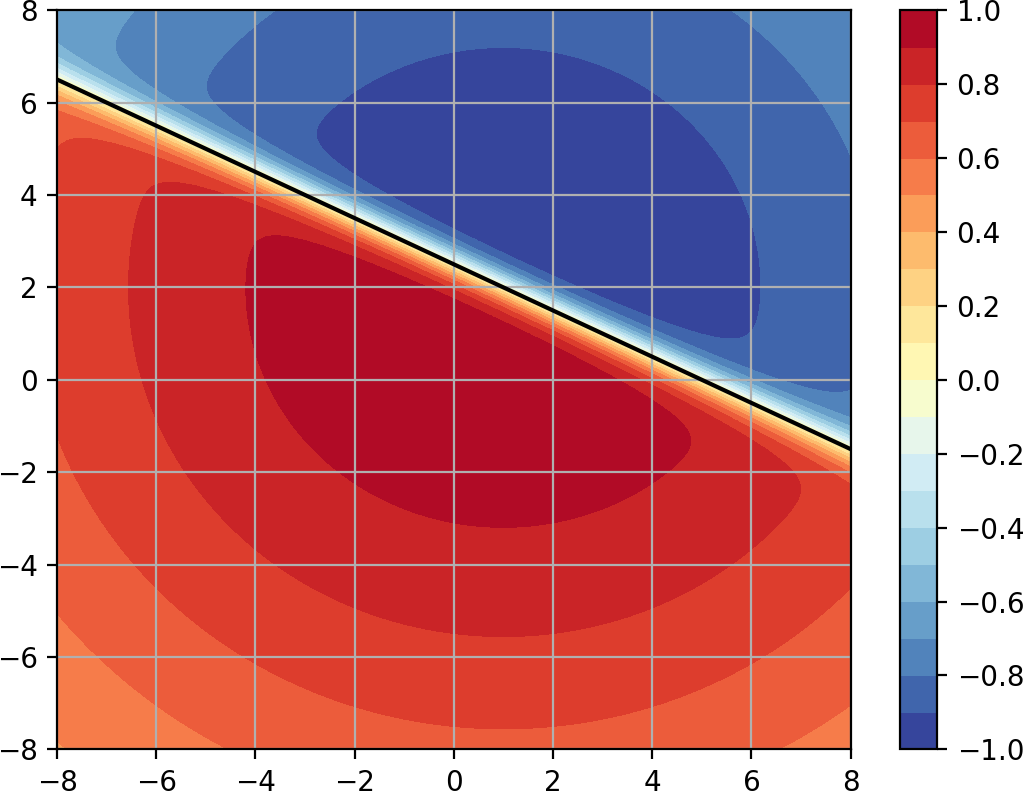
\includegraphics[height=3cm]{images/Matching-behavior/sigma-5-cropped.png}};\pause
        \node (img6)at(img5.south east) [xshift=-0.75cm]{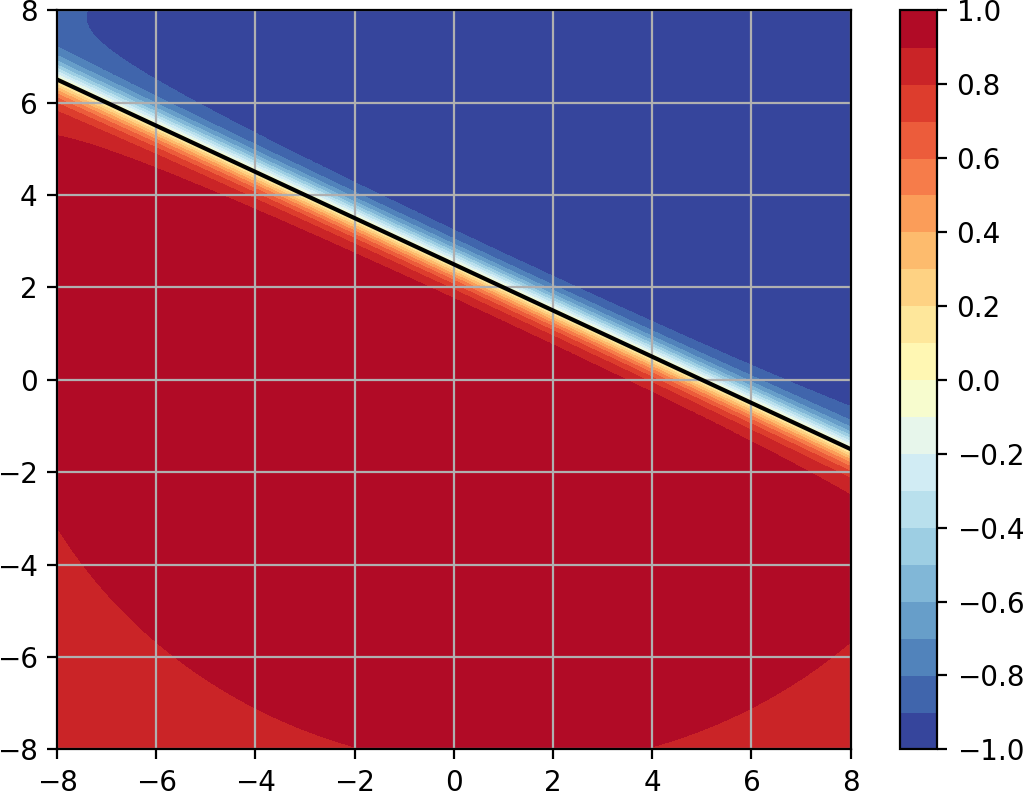
\includegraphics[height=3cm]{images/Matching-behavior/sigma-6-cropped.png}};\pause
        \node (img7)at(img6.north east) [xshift=-0.75cm]{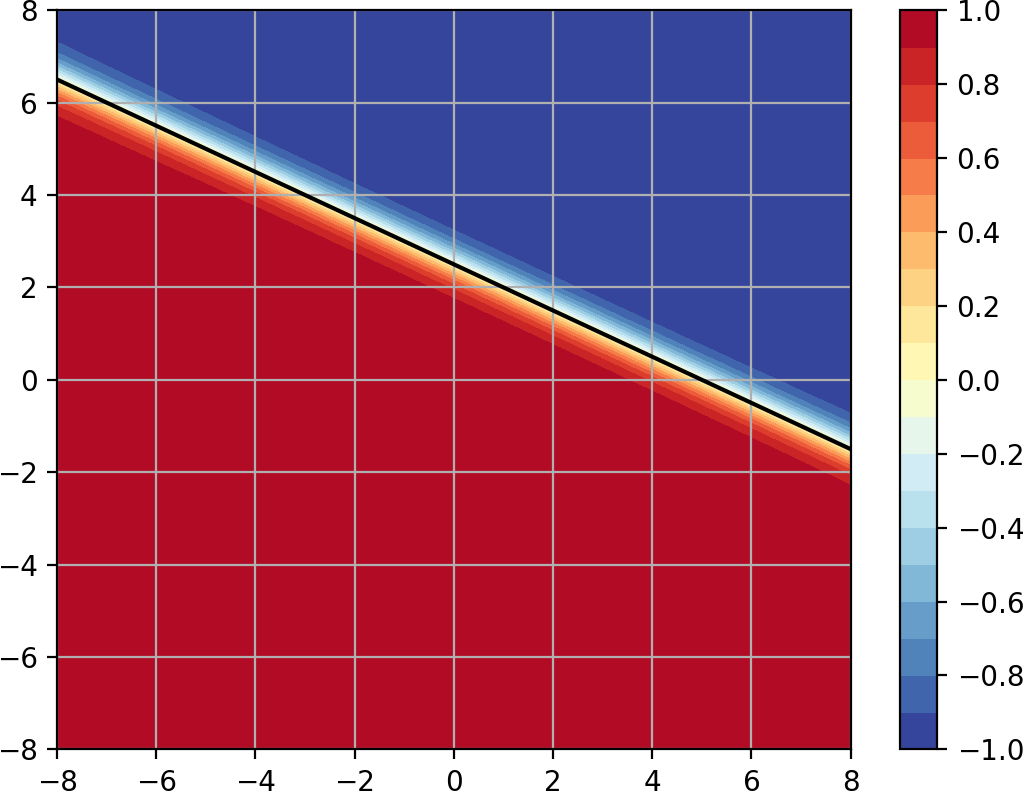
\includegraphics[height=3cm]{images/Matching-behavior/sigma-7-cropped.png}};
    \end{tikzpicture}
\end{frame}

\begin{frame}{Training the FGN}
    % talk about adapting SGD to the FGN math
    % adapt the loss function
    \begin{block}{Cost Function - Sigma Regularization}
    $$ C = C + \lambda\sigma^2  $$
    \end{block}
    
    \begin{block}{Gradients for Backpropagation}
    $$ y =  \varphi(\ell)*g = \tanh(\sum_i x_i w_i) * e^{\frac{-1}{\sigma^2}\sum_{i}(x_i-c_i)^2}$$
    \vspace{-0.6cm}
    \begin{align*}
        \frac{\partial y}{\partial w_i} &=  x_i \varphi'(\ell) * g  \\[1em]
        \frac{\partial y}{\partial c_i} &= \varphi(\ell) * \frac{2(x_i-c_i)}{\sigma^2} * g \\[1em]
        \frac{\partial y}{\partial \sigma} &= \varphi(\ell) * \frac{2\sum_{i}(x_i-c_i)^2}{\sigma^3}* g
    \end{align*}
    \end{block}
    \end{frame}
    
\begin{frame}{2D Toy Data - Single Neuron Training Sanity Check}
    \begin{columns}
    \begin{column}{.31\textwidth}
        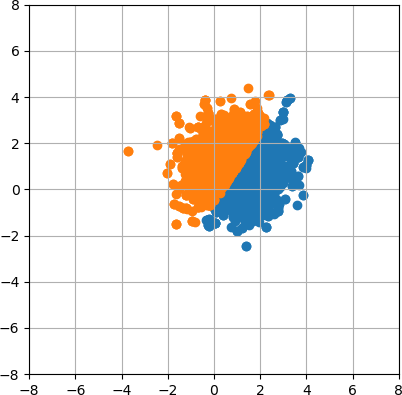
\includegraphics[width=0.85\textwidth]{images/2D-single-neuron/2d-easy-data-cropped.png}\\
        \centering\footnotesize{toy 2D data}
        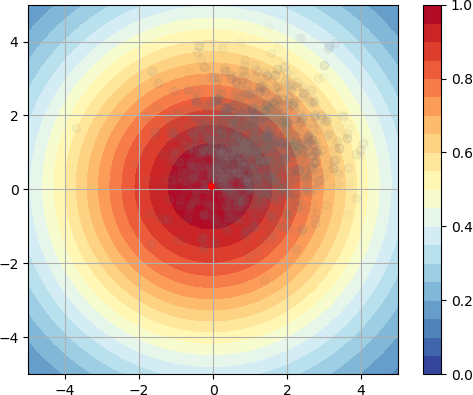
\includegraphics[width=\textwidth]{images/2D-single-neuron/2d-easy-initialg-cropped.png}
        \centering\footnotesize{$g$ pre-training}\\
    \end{column}
    
    \hspace{0.1cm}
    \begin{column}{.31\textwidth}
        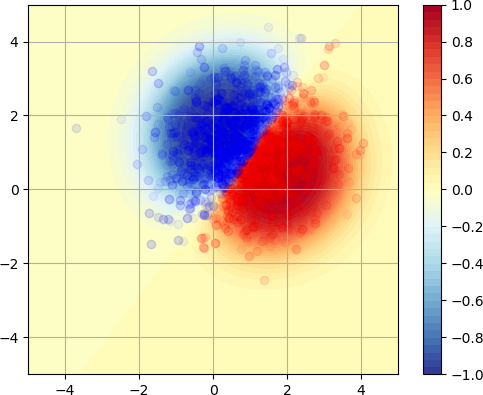
\includegraphics[width=1.02\textwidth]{images/2D-single-neuron/2d-easy-trained-activity-cropped.png}\\
        \centering\footnotesize{activity post-training}
        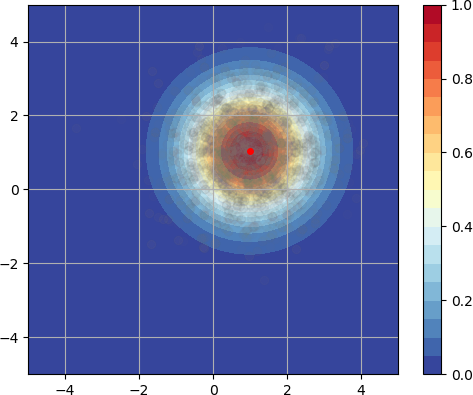
\includegraphics[width=\textwidth]{images/2D-single-neuron/2d-easy-trainedg-cropped.png}\\
         \centering\footnotesize{$g$ post-training}
    \end{column} 
    
    \hspace{0.1cm}
    \begin{column}{.31\textwidth}
        \vspace{0.1cm} \hspace{-0.01cm} 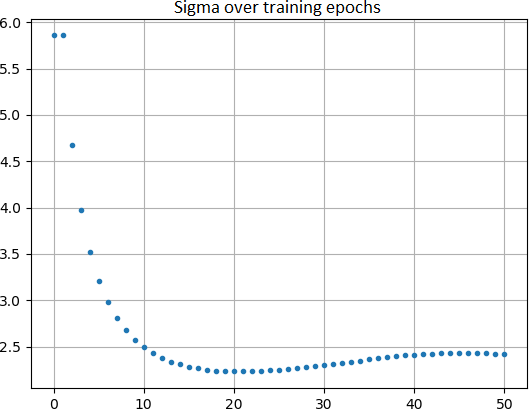
\includegraphics[width=0.84\textwidth,height=3.1cm]{images/2D-single-neuron/2d-easy-sigma-training-cropped.png}\\
        \centering\footnotesize{$\sigma$ over training}
        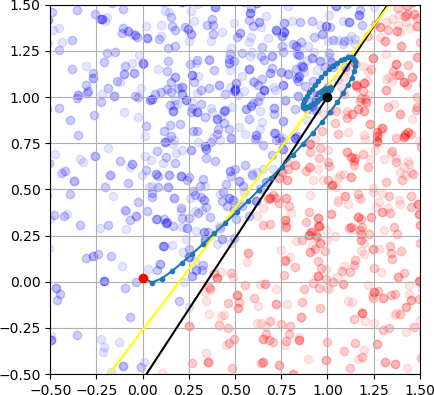
\includegraphics[width=0.92\textwidth]{images/2D-single-neuron/2d-easy-center-path-cropped.png}\\
        \centering\footnotesize{center path}
        
    \end{column}
    \end{columns}

\end{frame}

% \begin{frame}{Variants - Different $p$-norms}
%     \begin{block}{Gaussian Component with $p$-norm}
%         $$ g = e^{\frac{-1}{\sigma^2}\lVert x_i-c_i \lVert_p }$$
%     \end{block}
%     \vspace{0.3cm}
%     \begin{columns}
%     \hspace{-0.2cm}
%     \begin{column}{.27\textwidth}
%             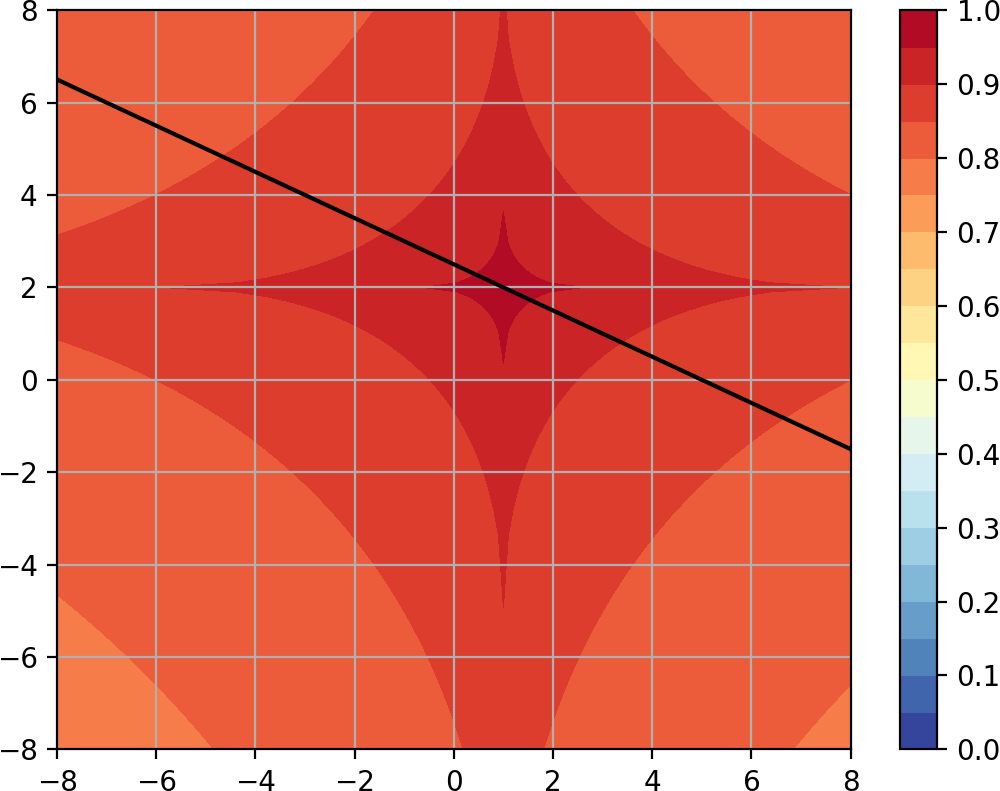
\includegraphics[width=\textwidth]{images/Variants-Norms/ord0.5_g-cropped.png}\\
%             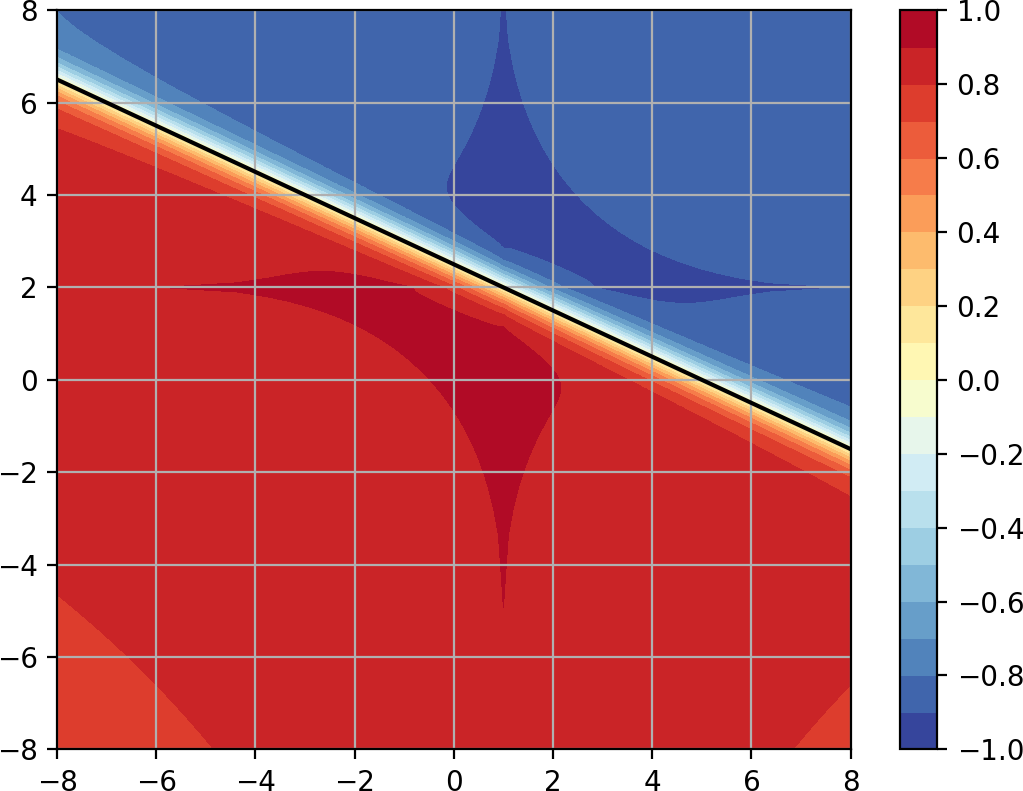
\includegraphics[width=\textwidth]{images/Variants-Norms/ord0.5-cropped.png}\\
%             \centering $p=0.5$
%     \end{column} \\
%     \hspace{0.1cm}
%     \begin{column}{.27\textwidth}
%             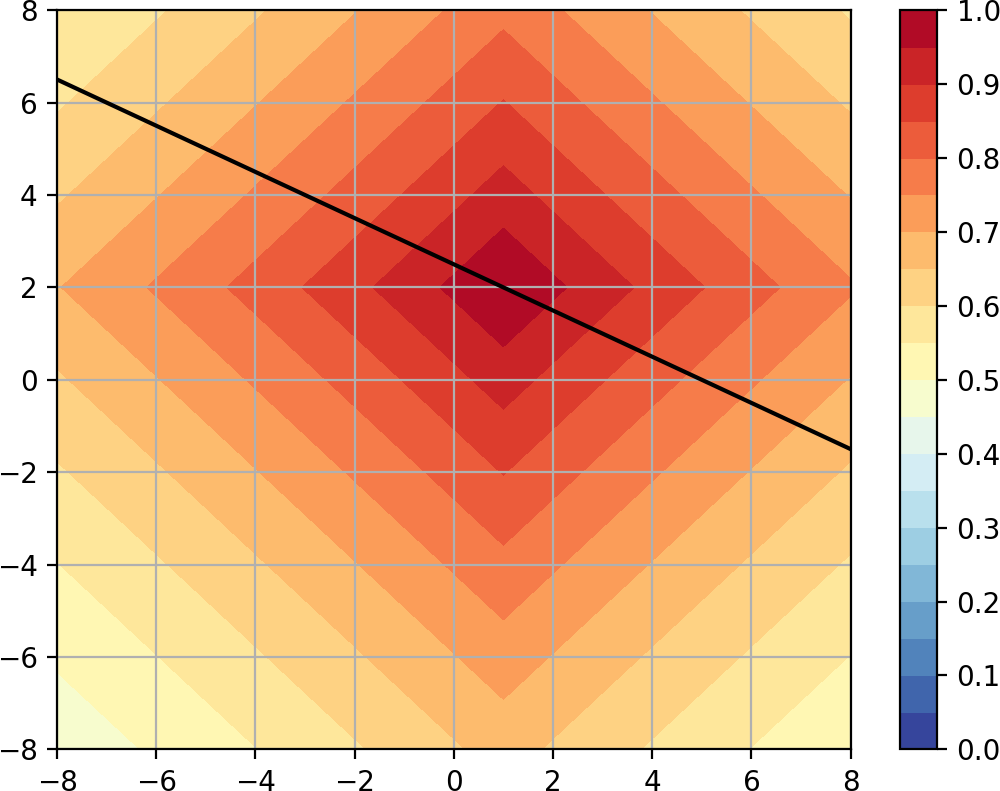
\includegraphics[width=\textwidth]{images/Variants-Norms/ord1_g-cropped.png}\\
%             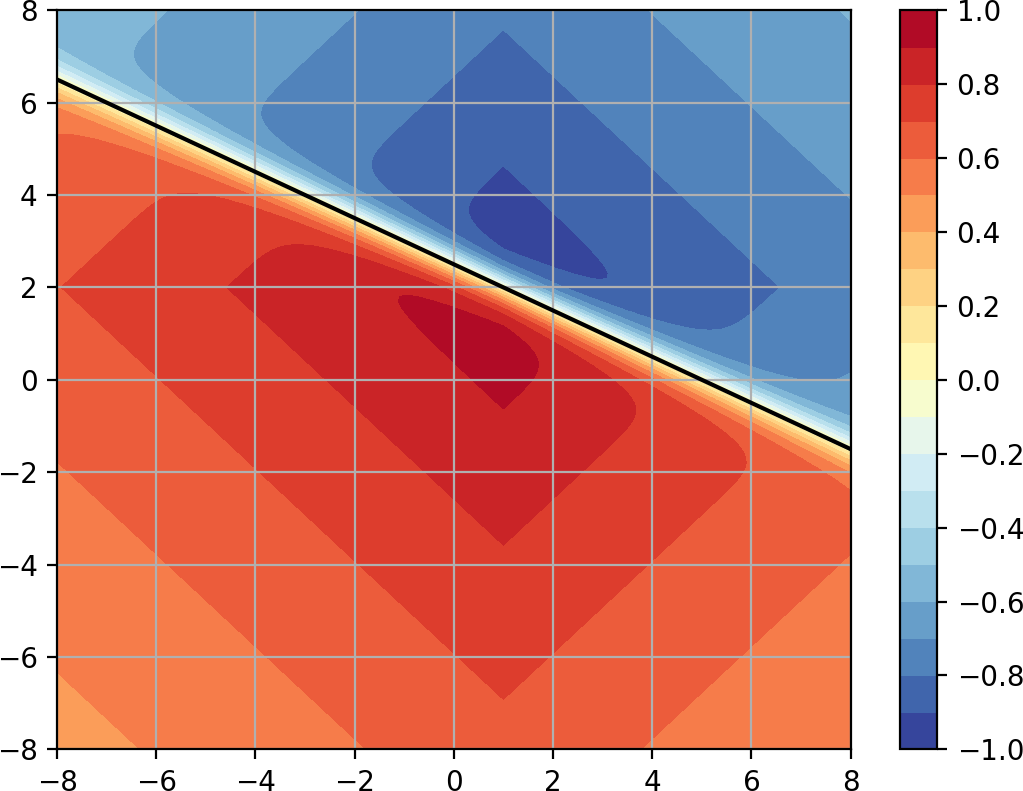
\includegraphics[width=\textwidth]{images/Variants-Norms/ord1-cropped.png}\\
%             \centering $p=1$
%     \end{column} \\
%     \hspace{0.1cm}
%     \begin{column}{.27\textwidth}
%             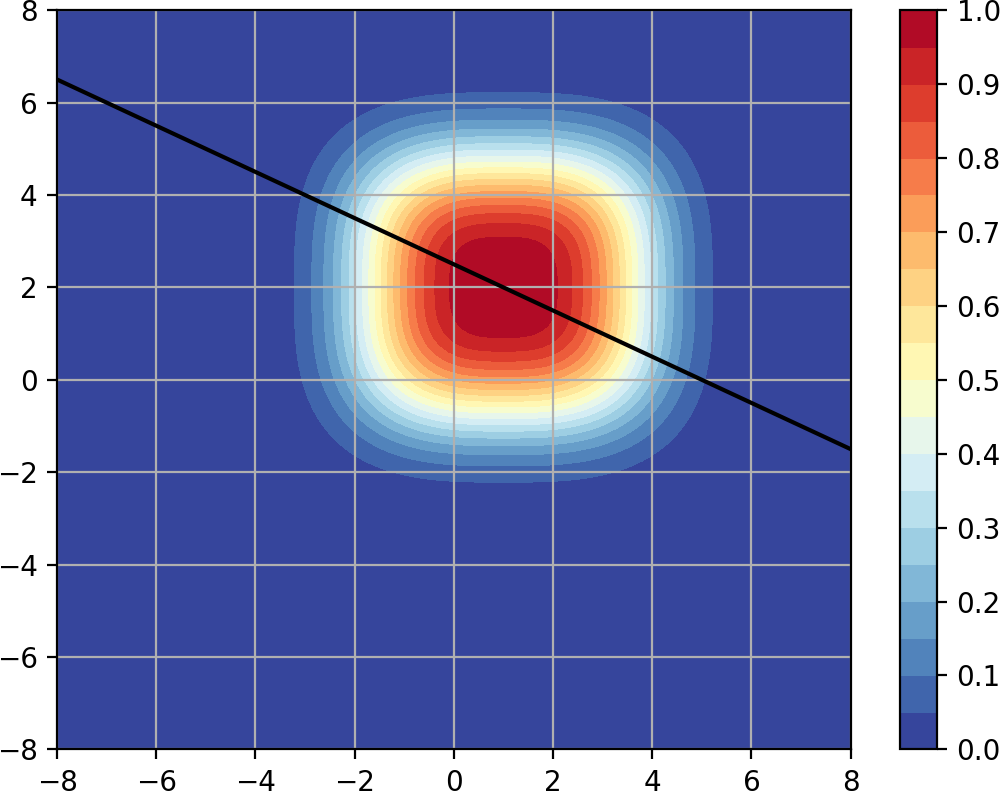
\includegraphics[width=\textwidth]{images/Variants-Norms/ord3_g-cropped.png}\\
%             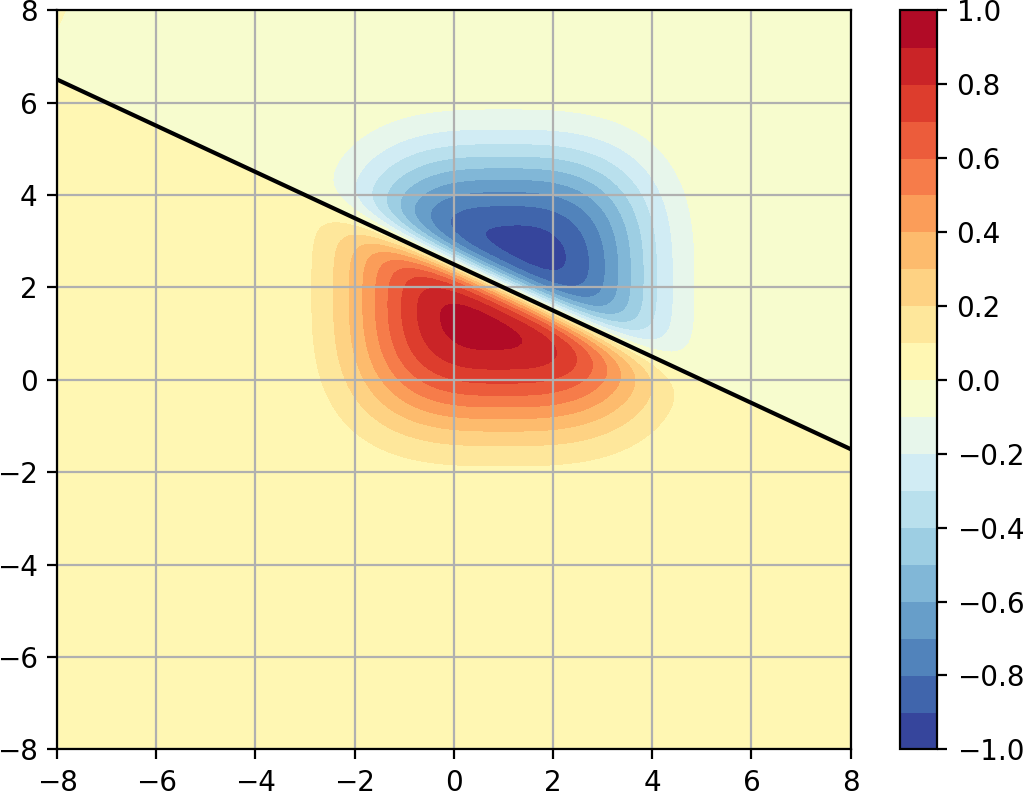
\includegraphics[width=\textwidth]{images/Variants-Norms/ord3-cropped.png}\\
%             \centering $p=3$
%     \end{column}
%     \end{columns}
% \end{frame}

\begin{frame}{Variants - Decoupled Bias/Centers}

    \begin{block}{}
    The default behavior is to have the bias of the linear term $\ell$ be \emph{unrestricted}: ie: not defined by the centers of the Gaussian term $g$.
    \end{block}
    
    \vspace{0.4cm}
    
    \centering
    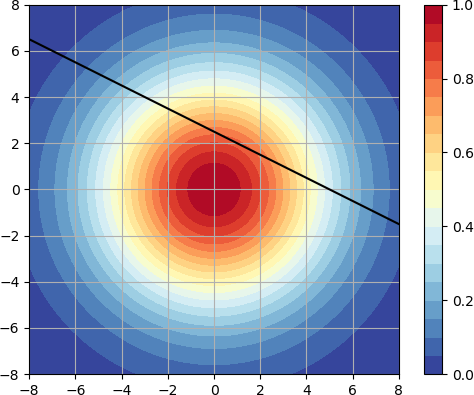
\includegraphics[height=0.5\textheight]{images/2D-Decoupled/var-decoupled-center-g-cropped.png}
    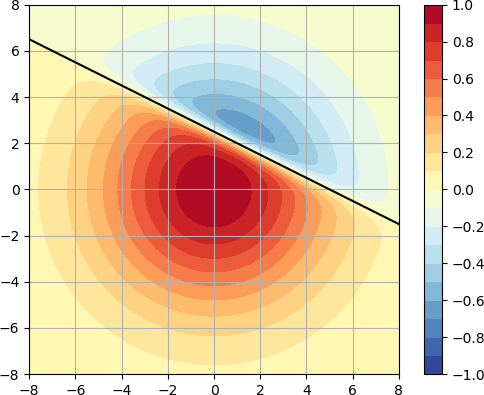
\includegraphics[height=0.5\textheight]{images/2D-Decoupled/var-decoupled-center-activity-cropped.png}\\
    
\end{frame}

\begin{frame}{Variants - Diagonal and Full Covariance}
    \begin{block}{Multivariate Gaussian Component}
    $$ g = e^{-(X-C)^T * \Sigma^{-1} * (X-C)}$$ \\
    with $X=[x_i]$ the inputs vector, $C=[c_i]$ the centers vector and $\Sigma$ the covariance matrix.
    \end{block}
    
    \begin{columns}
    \begin{column}{.5\textwidth}
    \begin{figure}
        \centering
        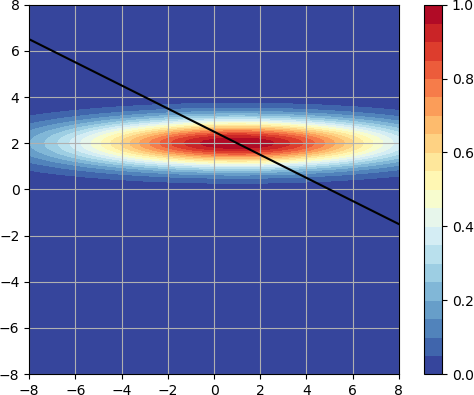
\includegraphics[width=0.81\textwidth]{images/Variants-Diag-Full-Cov/diag_g_activity_cropped.png}
        \caption*{Diagonal $\Sigma$}
    \end{figure}
    \end{column}
     \begin{column}{.5\textwidth}
    \begin{figure}
        \centering
        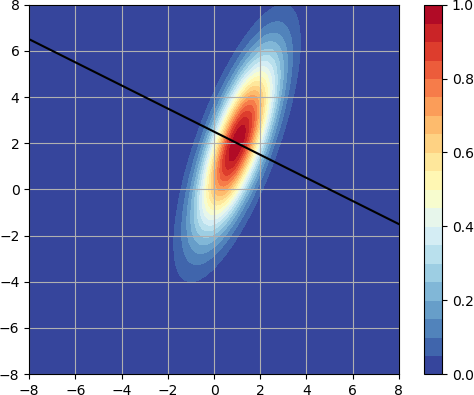
\includegraphics[width=0.81\textwidth]{images/Variants-Diag-Full-Cov/full_g_activity_cropped.png}
        \caption*{Full $\Sigma$}
    \end{figure}
    \end{column}
    \end{columns}
    
\end{frame}


\section{Multi-Layer Finite Gaussian Neural Networks}

\begin{frame}{Multi-Layer Finite Gaussian Neural Networks}
   \begin{block}{Layer $j$ Neuron Outputs}
        $$ y =  \varphi(\ell)*g = \varphi(\sum_i x_{i} w_{i}) * g $$\\[-0.2em]
        $$ g = \max(G_{j-1}) * e^{\frac{-1}{\sigma^2}\sum_{i}(x_i-c_i)^2}$$
        With $x_{i}$ and $G_{j-1}$ the previous layer outputs and Gaussian components.
    \end{block}
    
     \begin{center}
        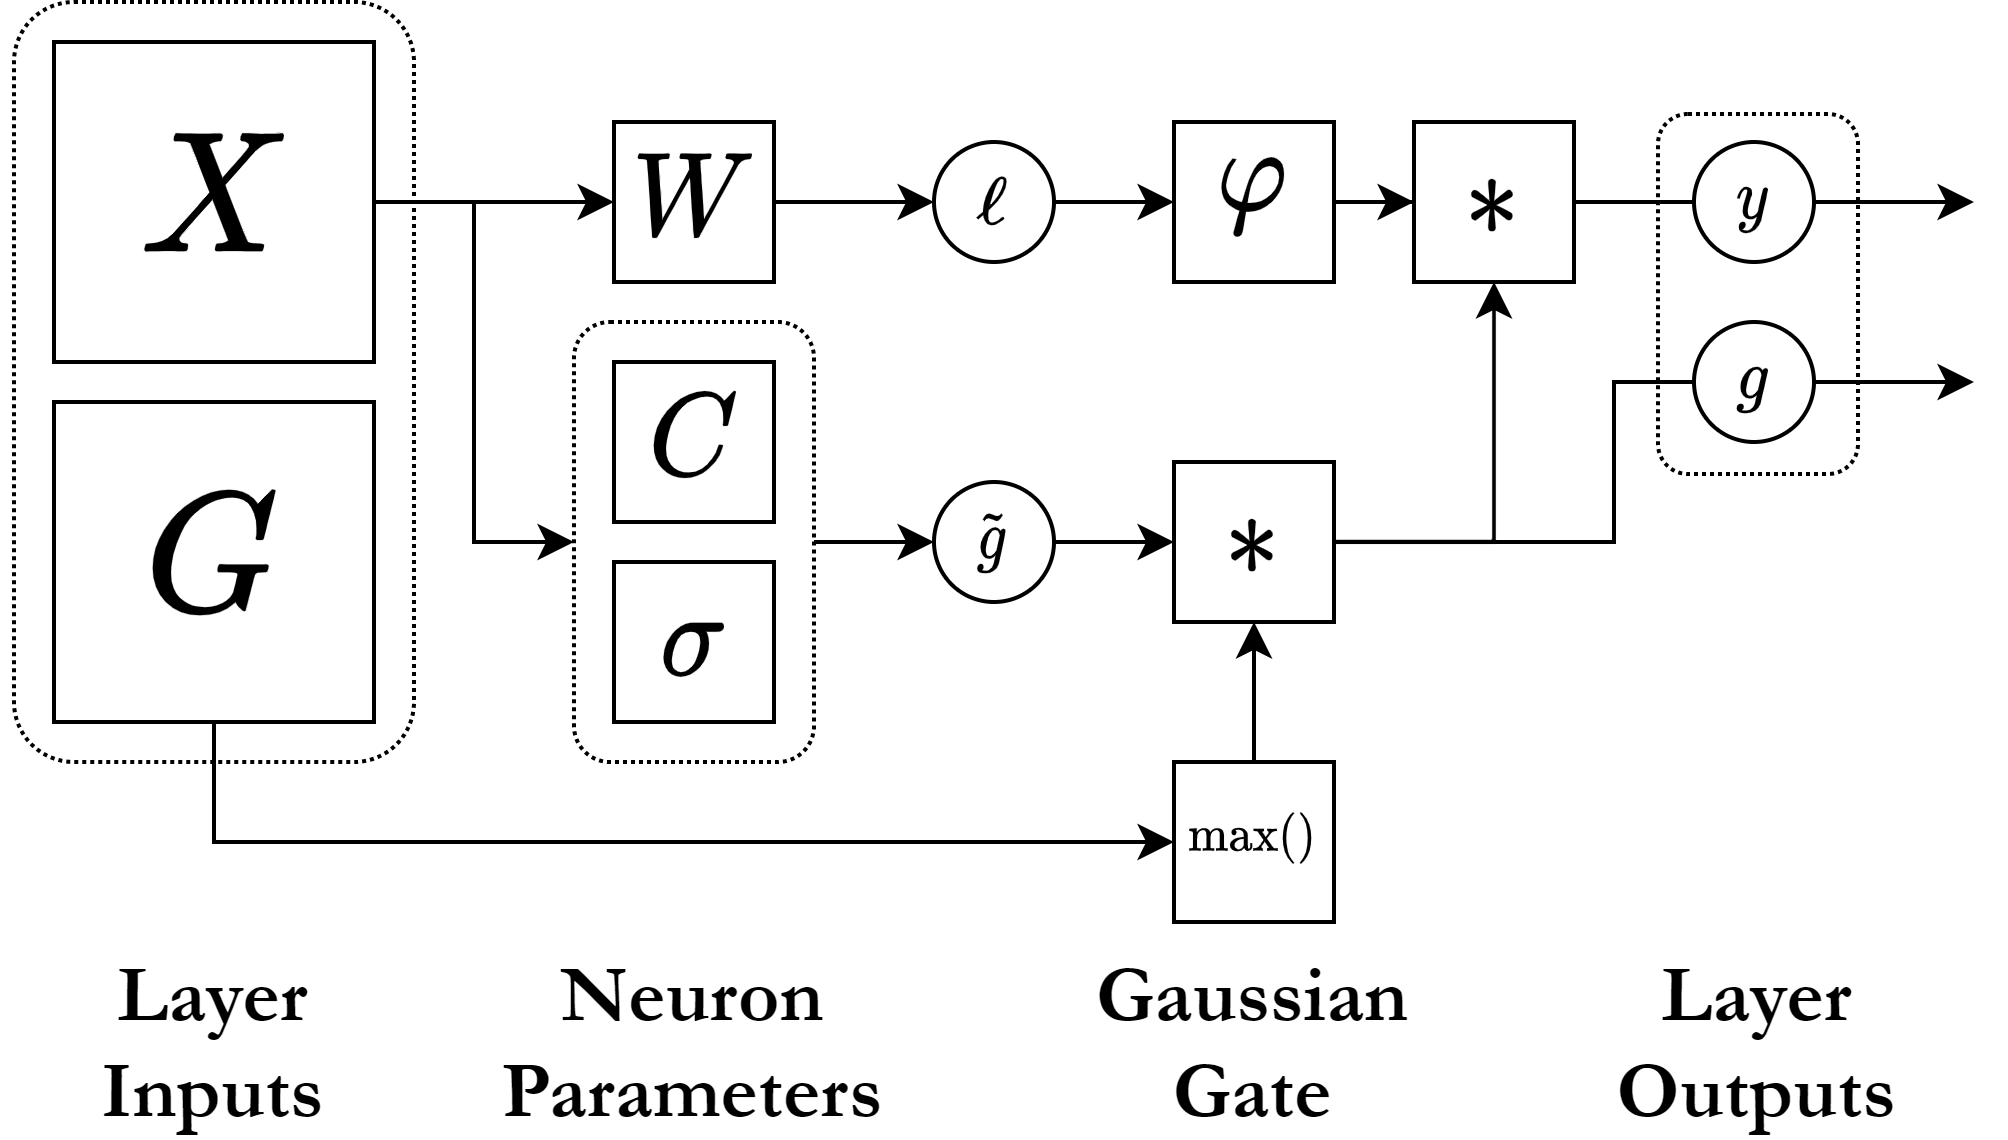
\includegraphics[width=0.6\textwidth]{images/multi-layer-fgn/FGN-Network.png}
    \end{center}

\end{frame}

\begin{frame}{2D Toy Data - Classic vs FGN Network}
    
    \vspace{-1cm}
    \begin{block}{}
    Activity of a classic feedforward network over 2D data, compared to that of an FGN network with the same number of neurons.
    \end{block}

    \begin{columns}
    \begin{column}{.333\textwidth}
    \vspace{2mm}
    \begin{figure}
        \centering
        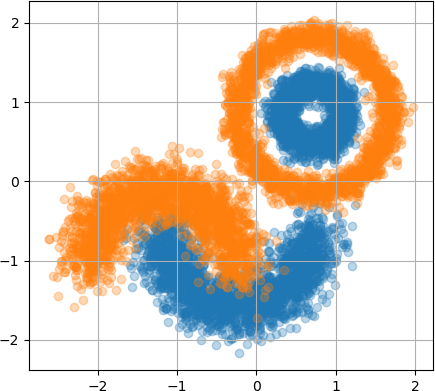
\includegraphics[width=0.92\textwidth]{images/2D-network-toy/2d-toy-data.png}
        \caption*{Toy Data}
    \end{figure}

    \end{column}
    \begin{column}{.333\textwidth}
    \begin{figure}
        \centering
        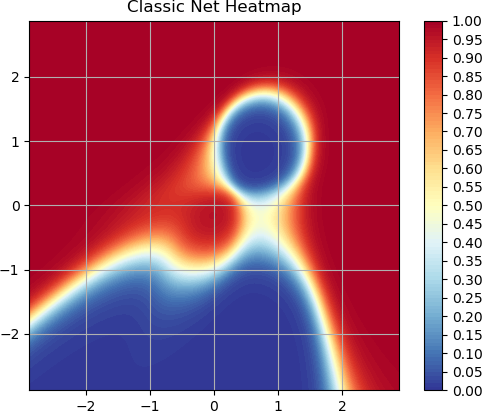
\includegraphics[width=1.\textwidth]{images/2D-network-toy/classic-heatmap.png}
        \caption*{Classic Net Activity}
    \end{figure}
    \end{column}
    \begin{column}{.333\textwidth}
    \begin{figure}
        \centering
        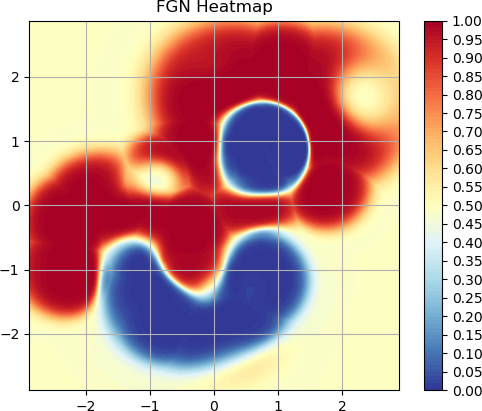
\includegraphics[width=1.\textwidth]{images/2D-network-toy/fgn-heatmap.png}
        \caption*{FGN Net Activity}
    \end{figure}
    \end{column}
    \end{columns}
    
\end{frame}

\begin{frame}{2D Toy Data - Classic vs FGN Network (continued)}
    \begin{columns}
    \begin{column}{.333\textwidth}
    \begin{figure}
        \centering
        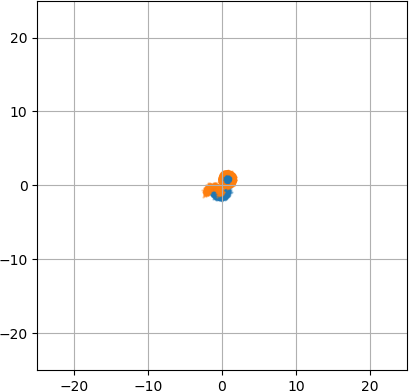
\includegraphics[width=0.92\textwidth]{images/2D-network-toy/2d-toy-data-zoomed-out.png}
        \caption*{Toy Data}
    \end{figure}
    \end{column}
    
    \begin{column}{.333\textwidth}
    \begin{figure}
        \centering
        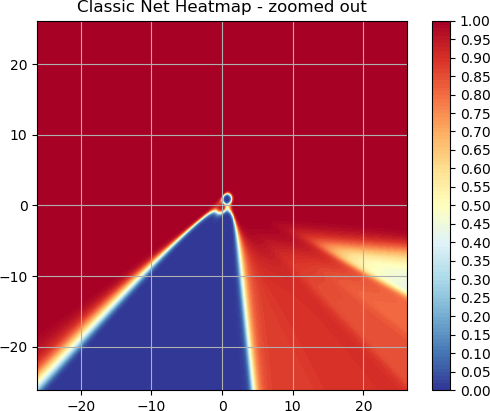
\includegraphics[width=1.\textwidth]{images/2D-network-toy/classic-heatmap-zoomed-out.png}
        \caption*{Classic Net Activity}
    \end{figure}
    \end{column}
    
    \begin{column}{.333\textwidth}
    \begin{figure}
        \centering
        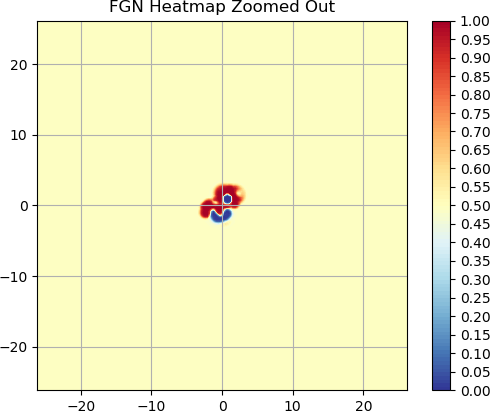
\includegraphics[width=1.\textwidth]{images/2D-network-toy/fgn-heatmap-zoomed-out.png}
        \caption*{FGN Net Activity}
    \end{figure}
    \end{column}
    \end{columns}
    
\end{frame}

\begin{frame}{2D Toy Data - Classic vs FGN Network (addendum)}
    
    \begin{block}{Training Parameters}
    $\bullet$ 32-16 neurons in hidden layers $\bullet$ spherical covariance $\bullet$ 2-norm $\bullet$ Adam optimizer $\bullet$ cross-entropy loss $\bullet$ 0.001 sigmas loss weight
    \end{block}

    \begin{columns}
    \begin{column}{.333\textwidth}
    \begin{figure}
        \centering
        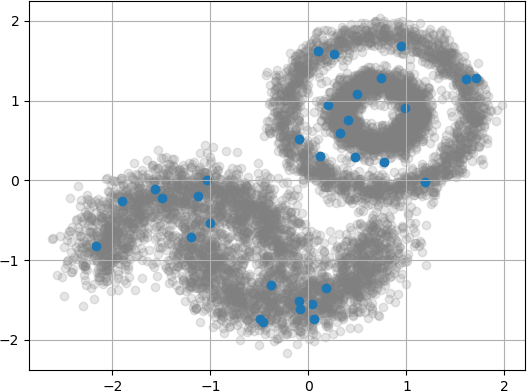
\includegraphics[width=1.\textwidth]{images/2D-network-toy/centers-init.png}
        \caption*{Initial Centers}
    \end{figure}
    \end{column}
    
    \begin{column}{.333\textwidth}
    \begin{figure}
        \centering
        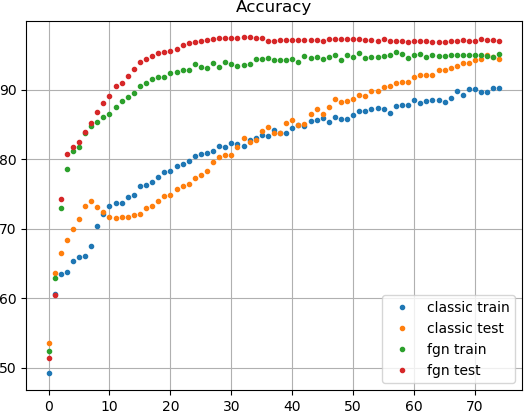
\includegraphics[width=1.\textwidth]{images/2D-network-toy/training-accuracy.png}
        \caption*{Training Accuracies}
    \end{figure}
    \end{column}
    
    \begin{column}{.333\textwidth}
    \begin{figure}
        \centering
        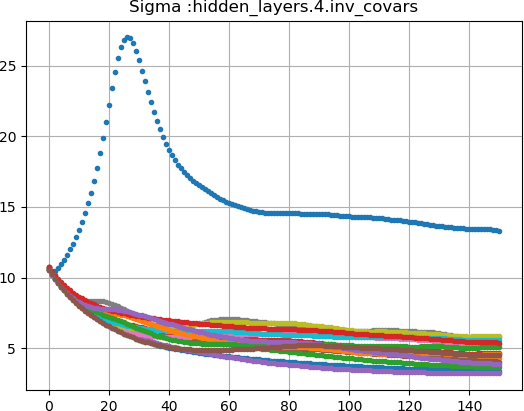
\includegraphics[width=1.\textwidth]{images/2D-network-toy/sigmas-change.png}
        \caption*{Sigmas Evolution}
    \end{figure}
    \end{column}
    \end{columns}
    
\end{frame}

\begin{frame}{2D Toy Data - Why is the Gaussian Gate Needed?}
    
    \vspace{-1mm}
    
    \begin{block}{}
        Without the Gaussian Gate, activity far from the data defaults to an arbitrary value, not necessarily zero. 
    \end{block}
    
    \begin{columns}
    \begin{column}{.48\textwidth}
    \begin{figure}
        \centering
        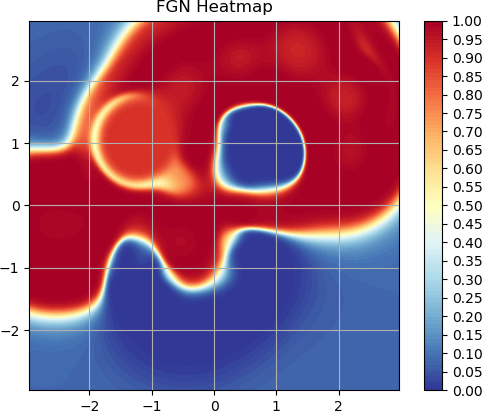
\includegraphics[width=1.\textwidth]{images/2D-network-toy/no-gate.png}
    \end{figure}
    \end{column}
    
    \begin{column}{.48\textwidth}
    \begin{figure}
        \centering
        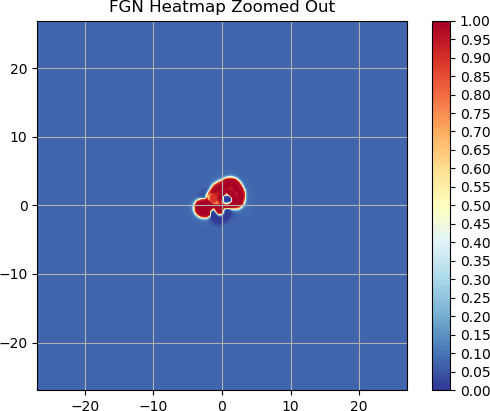
\includegraphics[width=1.\textwidth]{images/2D-network-toy/no-gate-zoomed-out.png}
    \end{figure}
    \end{column}
    \end{columns}

\end{frame}


\section{Networks over MNIST}

\begin{frame}{MNIST Behavior - Classic Network}
    \begin{columns}
    \begin{column}{.32\textwidth}
    \begin{figure}
        \centering
        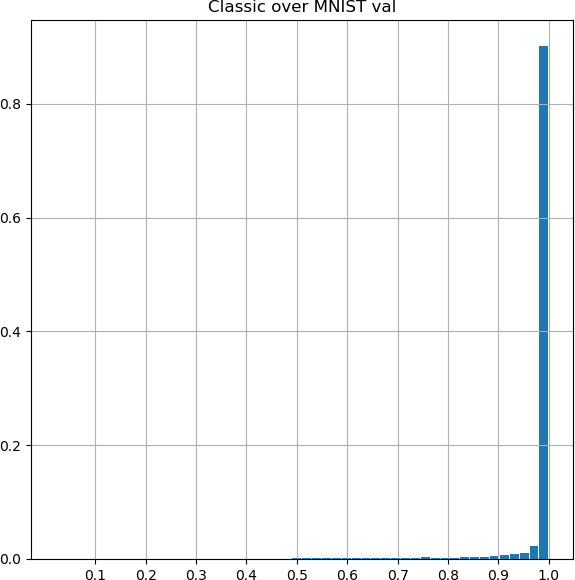
\includegraphics[width=.5\textwidth]{images/mnist-behavior/classic-hist-val.png}
    \end{figure}
        \begin{figure}
        \centering
        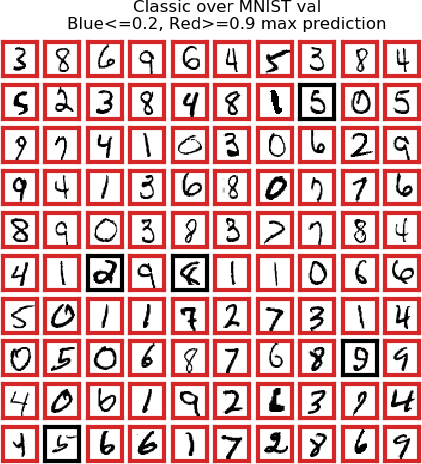
\includegraphics[width=.5\textwidth]{images/mnist-behavior/classic-pred-val.png}
    \end{figure}
    \end{column}
    
    \begin{column}{.32\textwidth}
    \begin{figure}
        \centering
        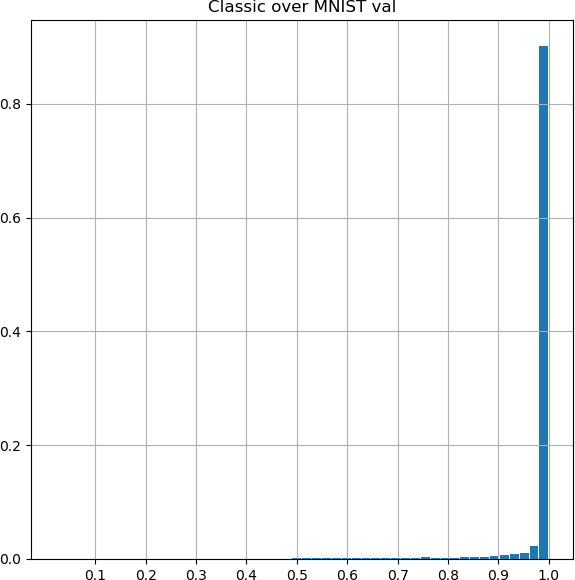
\includegraphics[width=.5\textwidth]{images/mnist-behavior/classic-hist-val.png}
    \end{figure}
        \begin{figure}
        \centering
        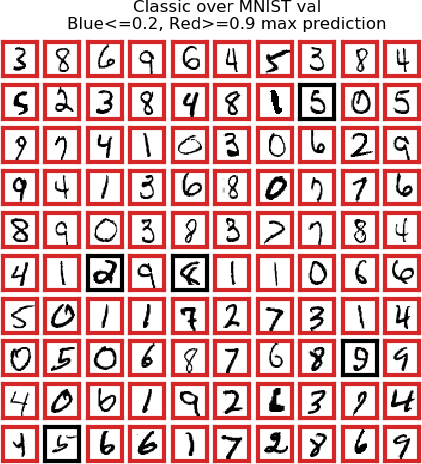
\includegraphics[width=.5\textwidth]{images/mnist-behavior/classic-pred-val.png}
    \end{figure}
    \end{column}
    
     \begin{column}{.32\textwidth}
    \begin{figure}
        \centering
        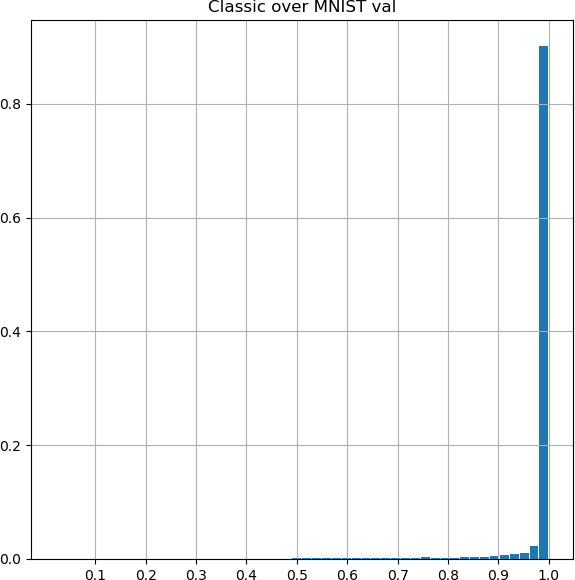
\includegraphics[width=.5\textwidth]{images/mnist-behavior/classic-hist-val.png}
    \end{figure}
        \begin{figure}
        \centering
        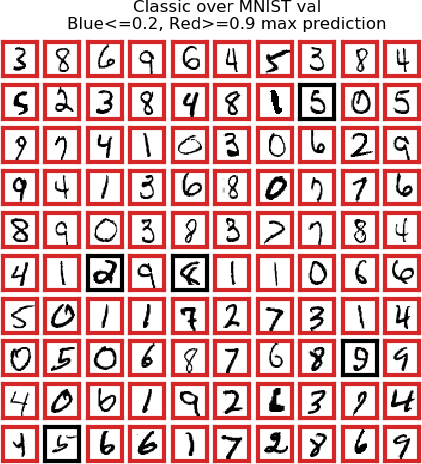
\includegraphics[width=.5\textwidth]{images/mnist-behavior/classic-pred-val.png}
    \end{figure}
    \end{column}
    
    \end{columns}
    
    
\end{frame}



\end{document}